%%
%% Template of the department Very Large Business Applications,
%%    CvO University Oldenburg for scientific papers
%%
%% Created by Dipl.-Inform. Daniel Süpke
%%    For questions, comments, suggestions etc. send an email to:
%%    suepke@wi-ol.de or suepke@gmx.de
%%
%% Version: April 16, 2010
%%
%% Note: Has only been tested with pdflatex, not latex (dvi). Still, there is
%% theoretical support also for latex.
%%
\documentclass[enabledeprecatedfontcommands,12pt]{scrartcl}

%% packages
\usepackage[utf8]{inputenc}       % Standard for Linux
%\usepackage[latin1]{inputenc}    % Standard for Windows
\usepackage{ngerman}              % For German language
\usepackage{fancyhdr}
\usepackage{geometry}
\usepackage{ifpdf}
\usepackage{setspace}             % For line spread
\usepackage[printonlyused, withpage, smaller]{acronym}

% For pdflatex
\ifpdf
  % One of these two:
  \usepackage[pdftex]{graphicx}
  %\usepackage[pdftex]{epsfig}

  \usepackage[pdftex]{hyperref}
% For latex (dvi)
\else
  % One of these two:
  \usepackage[dvips]{graphicx}
  %\usepackage[dvips]{epsfig}

  % make the command \href from hyperref available as a 'print only'
  \newcommand{\href}[2]{#2}
\fi

%% Picture options
\graphicspath{{pictures/}}         % Default path to pictures used
\DeclareGraphicsExtensions{.png}   % More extensions can be added

% Hyper ref coloring
\hypersetup{colorlinks, citecolor=black, linkcolor= black, urlcolor=black}

%% Pagestyle options
\pagestyle{fancy}
%\lhead{}
%\chead{}
%\rhead{}
%\lfoot{Daniel Süpke}
%\cfoot{}
%\rfoot{}
\renewcommand{\headrulewidth}{0.4pt}

\geometry{a4paper,left=3cm,right=3cm}
%\geometry{a4paper,left=3cm,right=2.5cm}   % Please use these settings for a PhD-thesis

%% Document start
\begin{document}

\pagenumbering{Roman}

% Insert titlepage
%% Title page
\begin{titlepage}
  \begin{centering}
  \begin{figure}[h!]
    \centering
    
\includegraphics[width=310pt]{CvO-Oldenburg-Logo}    % Ggf. Copyright beachten - ansonsten nur für Gebrauch an der CvO
  \end{figure}

  \vspace*{-0.8cm}

  \begin{figure}[h!]
    \centering
    
\includegraphics[width=250pt]{VLBA_waagerecht}    % Ggf. Copyright beachten - ansonsten nur für Gebrauch an der CvO/VLBA
  \end{figure}

  \vspace*{0.4cm}
  
  \textsf{\Huge \textbf{Cloud Computing, Internet of Things, Industrie 4.0, Predictive Maintenance, SCADA, SAP HANA\\}}

  \vspace*{0.5cm}
  \noindent Masterarbeit\\

  \end{centering}
  
  \vspace*{1.5cm}
  \begin{tabbing}
  xxxxxxxxxxxxxxxx\= \kill
  
  % Change me
  \small Themensteller:\> Prof. Dr.-Ing. Jorge Marx Gómez\\
  \small Betreuer:\> Prof. Dr.-Ing. Hergen Pargmann\\\\

  \small Vorgelegt von: \>Nils Lutz\\
  \small \>Erlenweg 5\\
  \small \>26129 Oldenburg\\
  \small \>+49 173 25 28 407\\
  \small \>nils.lutz@uni-oldenburg.de\\\\

  \small Abgabetermin:\> 30. April 2017
  \end{tabbing}
\end{titlepage}
%\thispagestyle{empty}
\newpage

% Insert table of contents
% Insert table of contents
\tableofcontents
\newpage

% Insert glossary, table of symbols, list of figures and list of tables
\section*{Akronyme}            % Alternatively a glossary package can be used
\addcontentsline{toc}{section}{Akronyme}
\begin{acronym}[HACCP]
  \acro{api}[API]{Application Programming Interface}
	\acro{baas}[BaaS]{Blockchain-as-a-Service}
  \acro{bft}[BFT]{Byzantine Fault Tolerant}
  \acro{bna}[BNA]{Business Network Archive}
  \acro{brc}[BRC]{British Retail Consortium}
	\acro{btc}[BTC]{Bitcoin}
  \acro{ca}[CA]{Certificate Authority}
  \acro{cli}[CLI]{Command Line Interface}
	\acro{dena}[dena]{Deutsche Energie-Agentur}
	\acro{dlt}[DLT]{Distributed Ledger Technology}
  \acro{dsgvo}[DSGVO]{Datenschutz-Grundverordnung}
  \acro{edi}[EDI]{Electronic Data Interchange}
  \acro{erp}[ERP]{Enterprise Resource Planning}
  \acro{gbt}[GBT]{Global Batch Traceability}
  \acro{gfsi}[GFSI]{Global Food Safety Initiative}
  \acro{gln}[GLN]{Global Location Number}
  \acro{gps}[GPS]{Global Positioning System}
  \acro{haccp}[HACCP]{Hazard Analysis and Critical Control Points}
  \acro{hmsc}[HMSC]{Halal Meat Supply Chain}
  \acro{http}[HTTP]{Hypertext Transfer Protocol}
  \acro{idoc}[IDoc]{Intermediate Document}
  \acro{ifs}[IFS]{International Food Standard}
  \acro{iln}[ILN]{Internationale Lokationsnummer}
	\acro{iot}[IoT]{Internet of Things}
  \acro{ki}[KI]{künstliche Intelligenz}
  \acro{lkv}[LKV]{Los-Kennzeichnungs-Verordnung}
  \acro{lmbg}[LMBG]{Lebensmittel- und Bedarfsgegenständegesetz}
  \acro{lmkv}[LMKV]{Lebensmittelkennzeichnungsverordnung}
	\acro{ml}[ML]{Machine Learning}
  \acro{msp}[MSP]{Member Ship Provider}
  \acro{pbft}[pBFT]{Practical Byzantine Fault Tolerant}
  \acro{pki}[PKI]{Public-Key-Infrastructure}
  \acro{poet}[PoET]{Proof-of-Elapsed-Time}
  \acro{pos}[PoS]{Proof-of-Stake}
  \acro{posp}[PoSp]{Proof-of-Space}
	\acro{pow}[PoW]{Proof-of-Work}
  \acro{reif}[REIF]{Resource-Efficent, Economic and Intelligent Foodchain}
  \acro{rest}[REST]{Representational State Transfer}
  \acro{rfid}[RFID]{Radiofrequenz-Identifikation}
	\acro{sc}[SC]{Smart Contract}
  \acro{sql}[SQL]{Structured Query Language}
  \acro{tls}[TLS]{Transport Layer Security}
  \acro{tms}[TMS]{Transportation Management System}
  \acro{ui}[UI]{User Interface}
  \acro{uri}[URI]{Uniform Resource Identifier}
  \acro{vvvo}[VVVO]{Vieh-Verkehrs-Verordnung}
  \acro{wms}[WMS]{Wharehouse Management System}
  \acro{xml}[XML]{Extensible Markup Language}
\end{acronym}

% \section*{Symbolverzeichnis}   % If needed
% \addcontentsline{toc}{section}{Symbolverzeichnis}
\newpage

\listoffigures
\addcontentsline{toc}{section}{Abbildungsverzeichnis}
\listoftables
\addcontentsline{toc}{section}{Tabellenverzeichnis}
\lstlistoflistings
\addcontentsline{toc}{section}{Quelltextverzeichnis}
\newpage


\pagenumbering{arabic}

%% Line spread
\onehalfspacing

% Insert introduction
\section{Motivation}

Industrie 4.0 ist ein Treiber der Digitalisierung vor allem im Bereich der Energiewirtschaft. \cite[vgl.]{UnternehmensbetreuungmbH2017} Durch den Einsatz von Industrie 4.0 sind Unternehmen in der Lage ihre Prozesse und Anlagen in Echtzeit Kontrollieren und Steuern zu können. Dadurch lassen sich Kosten optimieren und die Produktivität steigern. Industrie 4.0 ist der Oberbegriff für eine viel zahl von Technologien.\\
Eine Technologie die bereits heute neue innovative Ideen im privaten Sektor hervorgebracht hat, erobert den industriellen Sektor - Blockchain. Eine Blockchain ist eine verteilte Datenstruktur kombiniert mit Kryptographischen Methoden zur Sicherstellung der Unveränderbarkeit der Daten. Blockchains zählen zu den \ac{dlt}. So erwägen einige der größten Finanzinstitutionen den Einsatz von \ac{dlt}.\cite{Goldman2018}\cite{JPMorgan2018}\\

“Es ist davon auszugehen, dass wir in ein bis zwei Jahrzehnten wirtschaftlich über Mechanismen miteinander interagieren werden, für die wir bislang weder Konzepte noch Begriffe haben.” \cite[S.~92]{Platzer2014} Auch die Deutsche Bundesregierung ist an der Blockchain Technologie interessiert und erwägt den Einsatz in der Zukunft für die unterschiedlichsten Services. In einer der jüngsten Pressemitteilungen hat der Blockchain Bundesverband mitgeteilt, dass die Regierung eine umfassende Strategie zum Umgang und Einsatz der Technologie erarbeiten will. \cite{BCBundesverband2018}

\begin{figure}[h!]
	\centering
	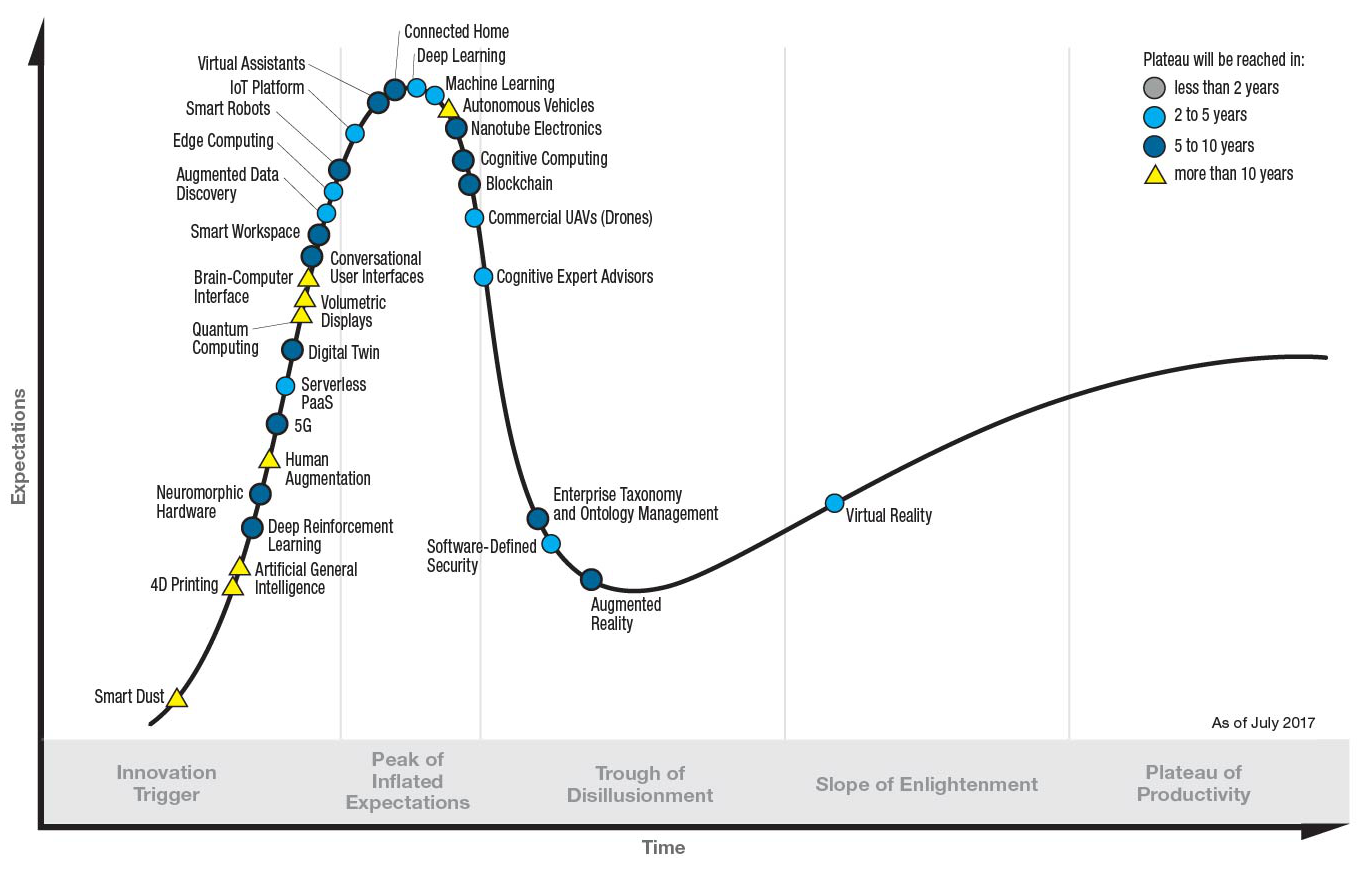
\includegraphics[width=0.65\linewidth]{pictures/Gartner-Hype-Cycle-2017}
	\caption[Gartner Hype Cycle 2017]{Emerging Technologies Hype Cycle 2017\cite{Gartner2017}}
	\label{fig:gartner-hype-cycle-2017}
\end{figure}

Noch ist die Blockchain kein Alltag, bemessen am jährlich erscheinenden Hype Cycle des Marktforschungsinstituts Gartner, Inc. $( Abb.~ \ref{fig:gartner-hype-cycle-2017} )$ hat die Technologie noch fünf bis zehn Jahre Entwicklungszeit vor sich. Erst dann wird sie nach aktueller Einschätzung im produktiven Einsatz sein. Was der Hype Cycle nicht aussagt ist welchen Einfluss die Blockchain auf eine Branche oder die Gesellschaft hat in ihrer jeweiligen Phase.\\

Bereits heute zeigen sich signifikante Unterschiede zwischen den unzähligen Blockchains die in Pilotprojekten realisiert wurden. So gibt es Anwendungen der Blockchain um beispielsweise den Kilometerstand eines Fahrzeugs täglich \glqq in die Blockchain\grqq~ zu schreiben. Die inhärenten Eigenschaften der Blockchain ermöglichen es sehr einfach festzustellen, ob ein Kilometerstand nachträglich durch Fremdeinwirkung manipuliert wurde. Ebenfalls ist keine zentrale Zwischenstelle mehr nötig, um für die Echtheit des hinterlegten Wertes zu garantieren. \cite{carVertical}\\

Bitcoin war die erste Generation von Blockchain. Die Bitcoin Blockchain ist in der Lage Einheiten der Bitcoin Währung zwischen zwei Parteien zu versenden ohne das eine Bank oder eine Clearingstelle diese Transaktion validieren muss. \cite[vgl.]{Nakamoto2009} Ethereum war die zweite Generation einer Blockchain. Im Vergleich zur Bitcoin Blockchain lassen sich mit dem Ethereum Netzwerk auch sog. \ac{sc} erstellen und ausführen.\cite[vgl.]{Buterin2014} Mittlerweile behaupten die ersten Projekte von sich zur dritten Generation von Blockchains zu gehören. Skalierbarkeit und Interoperabilität spielen in dieser Generation eine der entscheidenden Rollen. \cite[vgl.]{Cardano} Auch die Blockchain Anwendungen im Enterprise Bereich lassen in Masse noch auf sich warten. Es fehlen Erfahrungen und konkrete Einsatzgebiete für die Technologie.

\newpage


% Insert body
\section{Blockchain}
In diesem Grundlagen Kapitel soll ein Verständnis für die unterschiedlichen Begriffe und Verfahren der Blockchain Technologie etabliert werden. Beginnend mit einer allgemeinen Definition des Begriffs Blockchain, werden die verschiedenen Arten von \ac{dlt} im Detail betrachtet und definiert. Eine Abgrenzung zu Kryptowährungen soll zeigen, dass Blockchain nicht gleich Kryptowährungen bedeutet. In Kapitel 2.4 wird der technologische Hintergrund erörtert und abschließend soll eine Auflistung der vorhandenen \ac{dlt} die aktuelle Herstellerlandschaft zeigen.

\subsection{Definition}
Unter dem Begriff Blockchain wird eine Technologie verstanden, die eine erweiterbare Liste von Datensätzen bildet. Jeder Eintrag in dieser Liste wird Block genannt und ist durch kryptographische Methoden untereinander verkettet. Als Inhalt besitzt jeder Block einen kryptographischen Hashwert des vorhergehenden Blocks, sowie einen Zeitstempel und die eigentlichen Daten.\cite[Vgl.]{narayanan2016bitcoin} (Abbildung \ref{fig:simple-blockchain-schema})
\begin{figure}[h!]
	\centering
	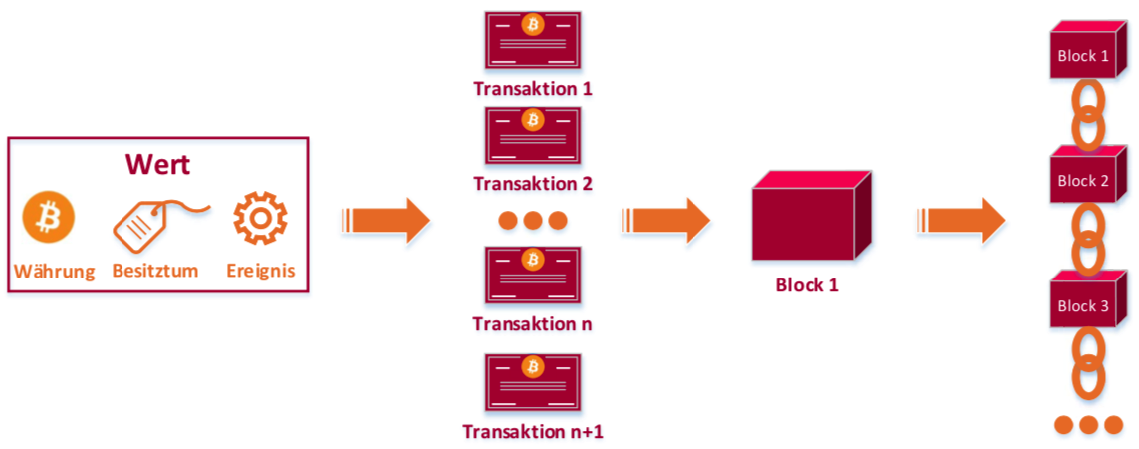
\includegraphics[width=1.0\linewidth]{pictures/simple-blockchain-schema}
	\caption[Vereinfachte Darstellung einer Blockchain]{Vereinfachte Darstellung einer Blockchain\cite{Gayvoronskaya2017}}
	\label{fig:simple-blockchain-schema}
\end{figure}

Technisch ist eine Blockchain also eine Art dezentrale Datenbank. Das Netzwerk aus Teilnehmern der Blockchain entscheidet im Konsens welcher Block (Datensatz) valide ist und der Gesamtmenge an Blöcken (Datenbank) angehangen wird. Zur Konsensbildung werden spezielle Algorithmen verwendet, um einen sog. byzantinischen Fehler zu verhindern. Durch die Vielzahl der Teilnehmer kann das mögliche Fehlermodell bei der Konsensbildung sehr komplex und schwer zu erfassen sein. Darauf beziehen sich byzantinische Fehler und die vorhandenen Lösungsansätze.

Der Oberbegriff \acf{dlt} wird in diesem Kontext gleichermaßen Synonym verwendet. Jedoch muss nicht zwingend jedes \glqq Distributed Ledger\grqq{} eine Blockchain als technische Grundlage verwenden. Viele unterschiedliche Ansätze werden aktuell in der Forschung und freien Marktwirtschaft erprobt und auf ihre Eigenschaften hin untersucht.

Das hohe Maß an Sicherheit, welches mit dem Begriff Blockchain assoziert wird, wird durch die Signierung der Blöcke und Transaktionen mit dem Public-Key-Verfahren garantiert. Auf dieses kryptographische Verfahren wird in Kapitel \ref{tec_bkgrnd_sec} näher eingegangen. In klassischen verteilten Datenbanken oder Systemen hat eine zentrale Organisation oder Kontrolleinheit als einzige die Möglichkeit den Datenbestand in einem konsistenten Zustand zu halten. Viel mehr ist diese zentrale Organisation der Vertrauensgeber des Systems - ohne Schutz vor Missbrauch. Um einem Missbrauch vorzubeugen sind \ac{dlt} dezentral organisiert. Dies bedeutet das es keine zentrale Einheit benötigt um Vertrauen über die Korrektheit der Transaktionen herzustellen.\cite[Vgl.]{Mitschele2018} (Abbildung \ref{fig:change-in-transaction-model-blockchain})
\begin{figure}[h!]
	\centering
	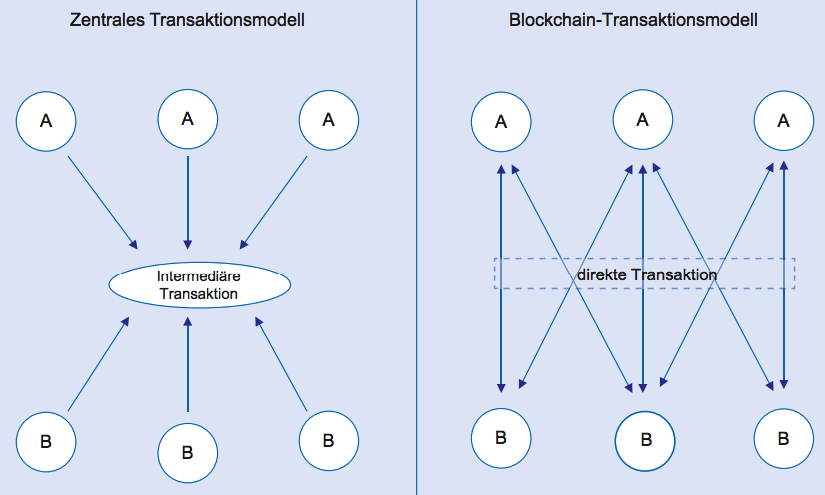
\includegraphics[width=0.81\linewidth]{pictures/change-in-transaction-model-blockchain}
	\caption[Veränderung des Transaktionsmodells durch die Blockchain]{Veränderung des Transaktionsmodells durch die Blockchain\cite{Kastrati2016}}
	\label{fig:change-in-transaction-model-blockchain}
\end{figure}

Die älteste sich noch in Betrieb befindliche \ac{dlt} ist die Blockchain der Kryptowährung \ac{btc}.

\subsection{Arten von \acl{dlt}}
Neben dem Blockchain Ansatz existieren noch weitere Ideen eines \ac{dlt}. Die aktuell am weitesten fortgeschrittenen Projekte sind der sog. \glqq Tangle\grqq{} von der Iota Foundation und die \glqq HashGraph\grqq{} genannte Technologie von Leemon Baird.\cite{Baird2016} Außerdem lassen sich \ac{dlt} in öffentlich-, privat- und konsortium Geführte Lösungen kategorisieren. Einige Ansätze lassen sich zu mehr als einer Kategorie zuordnen. Dies wird in den folgenden Unterkapiteln näher untersucht.

\subsubsection{Blockchain}
\begin{figure}[h!]
	\centering
	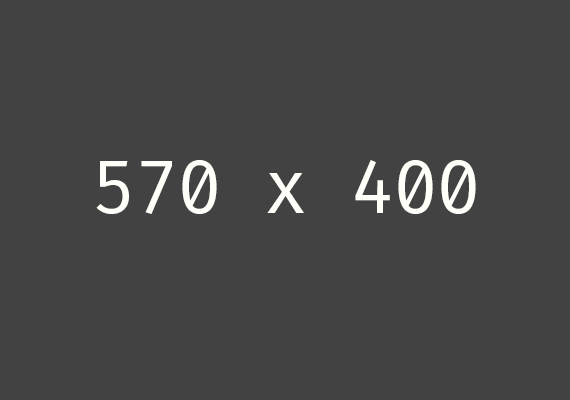
\includegraphics[width=1.0\linewidth]{pictures/placeholder_half_page}
	\caption[Placeholder Half Page]{Placeholder Half Page}
	\label{fig:placeholder_half_page}
\end{figure}


\subsubsection{Tangle}


\subsubsection{Hash Graph}
\begin{figure}[h!]
	\centering
	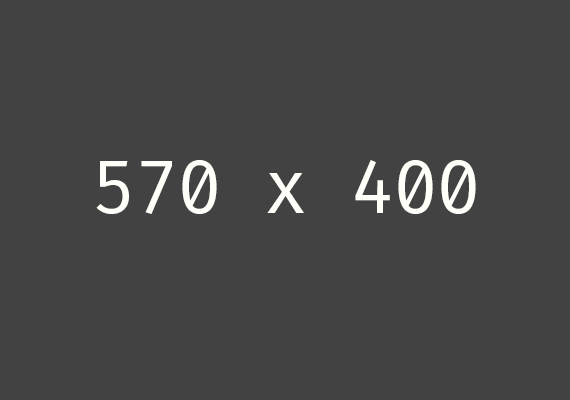
\includegraphics[width=1.0\linewidth]{pictures/placeholder_half_page}
	\caption[Placeholder Half Page]{Placeholder Half Page}
	\label{fig:placeholder_half_page}
\end{figure}


\subsubsection{Public}


\subsubsection{Private}


\subsubsection{Consortium}


\subsection{Abgrenzung Kryptowährungen}


\subsection{Technologischer Hintergrund}


\subsubsection{Sicherheit} \label{tec_bkgrnd_sec}


\paragraph{Public-Key Authorization}
\begin{figure}[h!]
	\centering
	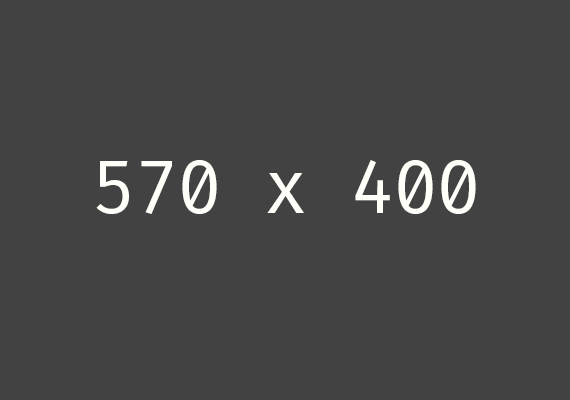
\includegraphics[width=1.0\linewidth]{pictures/placeholder_half_page}
	\caption[Placeholder Half Page]{Placeholder Half Page}
	\label{fig:placeholder_half_page}
\end{figure}


\paragraph{Hashing Algorithmus}


\subsubsection{Consensus Algorithmus}
\begin{figure}[h!]
	\centering
	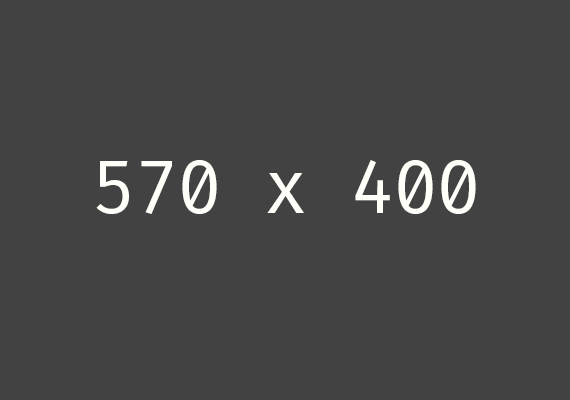
\includegraphics[width=1.0\linewidth]{pictures/placeholder_half_page}
	\caption[Placeholder Half Page]{Placeholder Half Page}
	\label{fig:placeholder_half_page}
\end{figure}


\paragraph{Proof-of-Work}
\begin{figure}[h!]
	\centering
	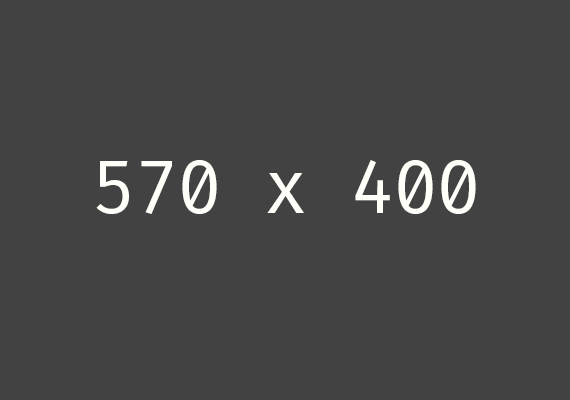
\includegraphics[width=1.0\linewidth]{pictures/placeholder_half_page}
	\caption[Placeholder Half Page]{Placeholder Half Page}
	\label{fig:placeholder_half_page}
\end{figure}


\paragraph{Proof-of-Stake}
\begin{figure}[h!]
	\centering
	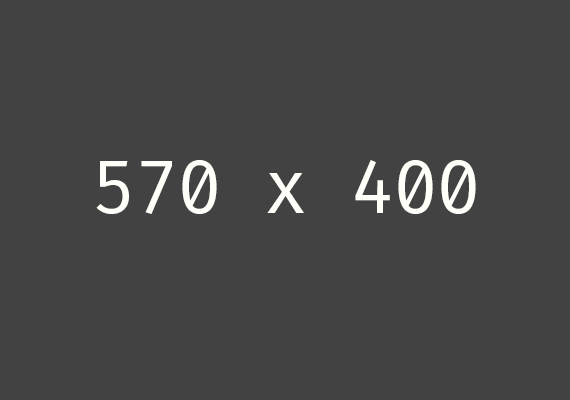
\includegraphics[width=1.0\linewidth]{pictures/placeholder_half_page}
	\caption[Placeholder Half Page]{Placeholder Half Page}
	\label{fig:placeholder_half_page}
\end{figure}


\paragraph{Delegated Proof-of-Stake}


\subsubsection{Peer-to-Peer Netzwerke}
\begin{figure}[h!]
	\centering
	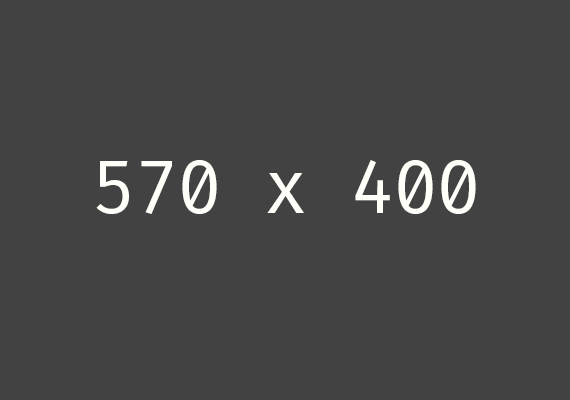
\includegraphics[width=1.0\linewidth]{pictures/placeholder_half_page}
	\caption[Placeholder Half Page]{Placeholder Half Page}
	\label{fig:placeholder_half_page}
\end{figure}


\subsubsection{Distributed Computing}


\subsection{Vorhandene Distributed Ledger}


\subsubsection{Bitcoin}


\subsubsection{Ethereum}


\subsubsection{IOTA}


\subsubsection{Ripple}


\subsubsection{IBM Bluemix}


\subsubsection{Microsoft Azure}


\subsubsection{Hyperledger Fabric}


\newpage
\section{Energiewirtschaft}

\subsection{Energieträger}

\subsubsection{Konventionelle}

\paragraph{Erdöl}

\paragraph{Kohle}

\paragraph{Erdgas}

\paragraph{Kernbrennstoff}

\subsubsection{Erneuerbare}

\paragraph{Wasser}

\paragraph{Sonne}

\paragraph{Wind}

\paragraph{Biomasse}

\subsection{Energiemarkt}

\subsubsection{Erzeuger}

\subsubsection{Konsumenten}

\subsubsection{Handel in Europa}

\paragraph{Börse}

\paragraph{OTC Handel}

\subsubsection{Deutschland}

\subsection{Wandel der Energiewirtschaft}

\subsubsection{Rechtliche Situation}

\subsubsection{Infrastruktur}

\subsubsection{Energiemix}
\begin{figure}[h!]
	\centering
	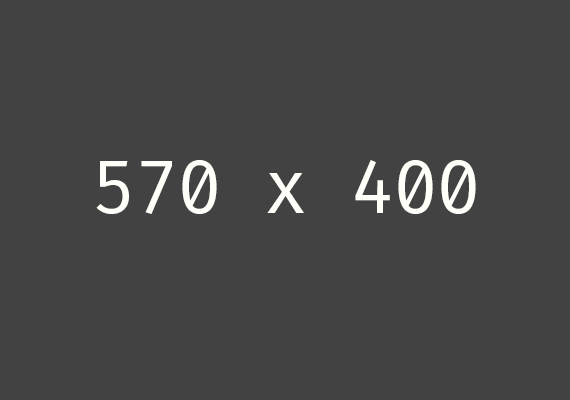
\includegraphics[width=1.0\linewidth]{pictures/placeholder_half_page}
	\caption[Placeholder Half Page]{Placeholder Half Page}
	\label{fig:placeholder_half_page}
\end{figure}

\subsubsection{Smart Grids und Smart Cities}

\subsection{Geschäftsmodelle}

\subsubsection{B2B}

\subsubsection{B2C}

\subsubsection{M2M}

\newpage
\section{Anwendungsgebiete für DLT in der Energiewirtschaft}

\subsection{Methoden zur Ermittlung der Anwendungsgebiete}

\subsubsection{SWOT-Analyse der Technologie}

\subsubsection{Entscheidungsbaum}

\subsection{Kriterien}

\subsubsection{Transaktional}

\subsubsection{Geschwindigkeit}

\subsubsection{Transparenz}

\subsubsection{Vertrauen}

\subsubsection{Unveränderlichkeit}

\subsubsection{Geschäftsregeln}

\subsection{Mehrwerte durch Distributed Ledger Technology}

\subsubsection{Transaktionskosten}

\subsubsection{Transaktionsgeschwindigkeit}

\subsubsection{Datenverfügbarkeit}

\subsubsection{Innovationskraft}

\subsection{Auswahl Geschäftsprozesse der Energiewirtschaft}

\subsubsection{Virtuelles Kraftwerk}

\subsubsection{Verwaltungsgesellschaft}

\subsubsection{Energiehandel}

\newpage
\section{Proof of Concept}

\subsection{Anforderungen DLT und Energiewirtschaft}

\subsection{Architektur}

\subsection{Entwicklung}

\newpage
\section{Auswertung}

\subsection{Kriterien}

\subsection{Abstraktionsmöglichkeit}

\newpage

% Insert conclusion
\section{Fazit}

Zwei flinke Boxer jagen die quirlige Eva und ihren Mops durch Sylt. Franz jagt im komplett verwahrlosten Taxi quer durch Bayern. Zwölf Boxkämpfer jagen Viktor quer über den großen Sylter Zwei flinke Boxer jagen die quirlige Eva und ihren Mops durch Sylt. Franz jagt im komplett verwahrlosten Taxi quer durch Bayern. Zwölf Boxkämpfer jagen Viktor quer über den großen Sylter Deich. Vogel Quax zwickt Johnys Pferd Bim. Sylvia wagt quick den Jux bei Pforzheim. Polyfon zwitschernd aßen Mäxchens Vögel Rüben, Joghurt und Quark.\\
"`Fix, Schwyz!"' quäkt Jürgen blöd vom Paß. Victor jagt zwölf Boxkämpfer quer über den großen Sylter Deich. Falsches Üben von Xylophonmusik quält jeden größeren Zwerg. Heizölrückstoßabdämpfung. Zwei flinke Boxer jagen die quirlige Eva und ihren Mops durch Sylt. Franz jagt im komplett verwahrlosten Taxi quer durch Bayern.\\
Zwölf Boxkämpfer jagen Viktor quer über den großen Sylter Deich. Vogel Quax zwickt Johnys Pferd Bim. Sylvia wagt quick den Jux bei Pforzheim. Polyfon zwitschernd aßen Mäxchens Vögel Rüben, Joghurt und Quark. "`Fix, Schwyz!"' quäkt Jürgen blöd vom Paß. Victor jagt zwölf Boxkämpfer quer über den großen Sylter Deich.\\

Falsches Üben von Xylophonmusik quält jeden größeren Zwerg. Heizölrückstoßabdämpfung. Zwei flinke Boxer jagen die quirlige Eva und ihren Mops durch Sylt. Franz jagt im komplett verwahrlosten Taxi quer durch Bayern. Zwölf Boxkämpfer jagen Viktor quer über den großen Sylter Deich. Vogel Quax zwickt Johnys Pferd Bim. Sylvia wagt quick den Jux bei Pforzheim.\\
Polyfon zwitschernd aßen Mäxchens Vögel Rüben, Joghurt und Quark. "`Fix, Schwyz!"' quäkt Jürgen blöd vom Paß. Victor jagt zwölf Boxkämpfer quer über den großen Sylter Deich. Falsches Üben von Xylophonmusik quält jeden größeren Zwerg. Heizölrückstoßabdämpfung. Zwei flinke Boxer jagen die quirlige Eva und ihren Mops durch Sylt. Franz jagt im komplett verwahrlosten Taxi quer durch Bayern. Zwölf Boxkämpfer jagen Viktor quer über den großen Sylter Deich. Vogel Quax zwickt Johnys Pferd Bim. Sylvia wagt quick den Jux bei Pforzheim. Polyfon zwitschernd aßen Mäxchens Vögel Rüben, Joghurt und Quark. "`Fix, Schwyz!"' quäkt Jürgen blöd vom Paß. Victor jagt zwölf\\

Zwei flinke Boxer jagen die quirlige Eva und ihren Mops durch Sylt. Franz jagt im komplett verwahrlosten Taxi quer durch Bayern. Zwölf Boxkämpfer jagen Viktor quer über den großen Sylter Deich. Vogel Quax zwickt Johnys Pferd Bim. Sylvia wagt quick den Jux bei Pforzheim. Polyfon zwitschernd aßen Mäxchens Vögel Rüben, Joghurt und Quark.\\
"`Fix, Schwyz"' quäkt Jürgen blöd vom Paß. Victor jagt zwölf Boxkämpfer quer über den großen Sylter Deich. Falsches Üben von Xylophonmusik quält jeden größeren Zwerg. Heizölrückstoßabdämpfung. Zwei flinke Boxer jagen die quirlige Eva und ihren Mops durch Sylt. Franz jagt im komplett verwahrlosten Taxi quer durch Bayern.\\
Zwölf Boxkämpfer jagen Viktor quer über den großen Sylter Deich. Vogel Quax zwickt Johnys Pferd Bim. Sylvia wagt quick den Jux bei Pforzheim. Polyfon zwitschernd aßen Mäxchens Vögel Rüben, Joghurt und Quark. "`Fix, Schwyz"' quäkt Jürgen blöd vom Paß. Victor jagt zwölf Boxkämpfer quer über den großen Sylter Deich.\\

Falsches Üben von Xylophonmusik quält jeden größeren Zwerg. Heizölrückstoßabdämpfung. Zwei flinke Boxer jagen die quirlige Eva und ihren Mops durch Sylt. Franz jagt im komplett verwahrlosten Taxi quer durch Bayern. Zwölf Boxkämpfer jagen Viktor quer über den großen Sylter Deich. Vogel Quax zwickt Johnys Pferd Bim. Sylvia wagt quick den Jux bei Pforzheim.\\
Polyfon zwitschernd aßen Mäxchens Vögel Rüben, Joghurt und Quark. "`Fix, Schwyz"' quäkt Jürgen blöd vom Paß. Victor jagt zwölf Boxkämpfer quer über den großen Sylter Deich. Falsches Üben von Xylophonmusik quält jeden größeren Zwerg. Heizölrückstoßabdämpfung. Zwei flinke Boxer jagen die quirlige Eva und ihren Mops durch Sylt. Franz jagt im komplett verwahrlosten Taxi quer durch Bayern. Zwölf Boxkämpfer jagen Viktor quer über den großen Sylter Deich. Vogel Quax zwickt Johnys Pferd Bim. Sylvia wagt quick den Jux bei Pforzheim. Polyfon zwitschernd aßen Mäxchens Vögel Rüben, Joghurt und Quark. "`Fix, Schwyz"' quäkt Jürgen blöd vom Paß. Victor jagt zwölf

\newpage

\pagenumbering{Roman}
\setcounter{page}{7}

% Insert appendix
\begin{appendix}

\section{Anhang}
Weitere Informationen werden im Anhang abgedruckt (z. B. Listings).

\begin{verbatim}
10 PRINT "Sales and Distribution"
20 GOTO 10
\end{verbatim}

\newpage
Das Literaturverzeichnis ist Bestandteil jeder wissenschaftlichen Arbeit. Präzise und aussagekräftige Angaben erleichtern die Recherche für spätere Leser. Die Verwendung von Zitaten oder Ideen aus anderen Arbeiten oder aus sonstigen Quellen ohne deutlichen Hinweis auf deren Ursprung stellt eines der schwersten akademischen Vergehen dar. Eine wissenschaftliche Arbeit, in der dieser Fehler wiederholt gemacht wird, wird zu Recht als Plagiat bezeichnet.
\addcontentsline{toc}{section}{Literaturverzeichnis}
\bibliographystyle{alpha}
\bibliography{thesis} % Point to BibTeX literature file e.g. literatur.bib

\end{appendix}
\newpage


% Insert declaration
\section*{Abschließende Erklärung}

Ich versichere hiermit, dass ich meine Masterarbeit selbständig und ohne fremde Hilfe angefertigt habe, und dass ich alle von anderen Autoren wörtlich übernommenen Stellen wie auch die sich an die Gedankengänge anderer Autoren eng anlegenden Ausführungen meiner Arbeit besonders gekennzeichnet und die Quellen zitiert habe.

\vspace*{3cm}
\noindent Oldenburg, den \today \hspace*{2cm} Nils Lutz


\end{document}
